\documentclass[10pt]{article}
\usepackage[utf8]{inputenc}
\usepackage[T1]{fontenc}
\usepackage{amsmath}
\usepackage{amsfonts}
\usepackage{amssymb}
\usepackage{mhchem}
\usepackage{stmaryrd}
\usepackage{graphicx}
\usepackage[export]{adjustbox}
\graphicspath{ {./images/} }
\usepackage{bbold}
\usepackage{hyperref}
\hypersetup{colorlinks=true, linkcolor=blue, filecolor=magenta, urlcolor=cyan,}
\urlstyle{same}

\begin{document}
\section{Contents}
1 Convolutional Neural Networks $\ldots \ldots \ldots \ldots \ldots \ldots \ldots$

$1.1$ Convolutional operations $\ldots \ldots \ldots \ldots \ldots \ldots \ldots \ldots \ldots$

1.1.1 Images as matrix $\ldots \ldots \ldots \ldots \ldots . . . . . . . . . . . . . . . . .$

1.1.2 Convolution operation with one channel $\ldots \ldots \ldots \ldots \ldots .$

1.1.3 Convolution with stride (one channel) $\ldots \ldots \ldots \ldots \ldots \ldots .$

1.1.4 Convolutional operations with multi-channel $\ldots \ldots \ldots \ldots .6$

$1.1 .5$ Pooling operation in CNNs $\ldots \ldots . \ldots . . . . . . . . . . . . . . . . .$

$1.2$ Examples of convolution filters and performance $\ldots \ldots \ldots \ldots, \ldots$

1.2.1 Calculation with convolutions .............................. 8

$1.2 .2 \quad$ Image convolution examples $\ldots \ldots \ldots \ldots . \ldots . . . . . . . . . .$

1.2.3 Line detection by 1D Laplacian $\ldots \ldots \ldots . \ldots . . . . . . . . .$

1.2.4 Edge detection by 2D Laplacian operator $\ldots \ldots \ldots \ldots \ldots .12$

1.2.5 The Laplacian of Gaussian $\ldots \ldots \ldots \ldots . . . . . . . . . . . .$

1.2.6 Other examples with ReLU activation $\ldots \ldots \ldots \ldots \ldots .15$

1.2.7 Some other examples $\ldots \ldots \ldots \ldots \ldots \ldots \ldots . . . . . . . . . . . . . . . . . . .$

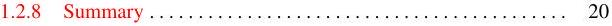
\includegraphics[max width=\textwidth]{2022_01_06_b5ce182ed1bd5f482e5bg-01}

References $\ldots \ldots \ldots \ldots \ldots \ldots \ldots \ldots \ldots \ldots \ldots \ldots \ldots \ldots$


\includegraphics[max width=\textwidth]{2022_01_06_b5ce182ed1bd5f482e5bg-02}

\section{Convolutional Neural Networks}
\subsection{Convolutional operations}
\subsubsection{Images as matrix}
An image can be viewed as a piecewise constant function on a grid. Images with different resolutions can then be viewed as functions on grids of different sizes. The use of such multiple-grids is a main technique used in the standard multigrid method for solving discretized partial differential equations, and it can also be interpreted as a main ingredient used in convolutional neural networks (CNN) for image calssification.

An image can be viewed as a function on a grid [6] on a rectangle domain $\Omega \in \mathcal{R}^{2}$. Without loss of generality, we assume that the grid, $\mathcal{T}$, is of size
$$
m=2^{s}, \quad n=2^{t}
$$
for some integers $s, t \geq 1$. Starting from $\mathcal{T}_{1}=\mathcal{T}$, we consider a sequence of coarse grids with $J=\min (s, t)$ (as depicted in Fig. 1.1.1 with $J=4)$ :
$$
\mathcal{T}_{1}, \mathcal{T}_{2}, \ldots, \mathcal{T}_{J}
$$
such that $\mathcal{T}_{\ell}$ consist of $m_{\ell} \times n_{\ell}$ grid points, with
$$
m_{\ell}=2^{s-\ell+1}, \quad n_{\ell}=2^{t-\ell+1} .
$$
Here, please note that each element in this grid can be viewed as a pixel or an image or an element in a matrix.

\subsubsection{Convolution operation with one channel}
For simplicity of exposition, we denote
$$
m=m_{1}=2^{s}, \quad n=n_{1}=2^{t} .
$$
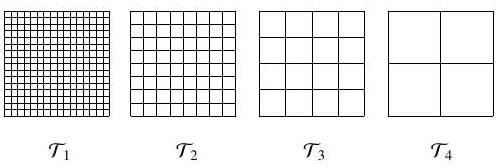
\includegraphics[max width=\textwidth]{2022_01_06_b5ce182ed1bd5f482e5bg-04}

Fig. 1.1. multilevel grids for piecewise constant functions (images)

Definition 1. A convolution defined on $\mathbb{R}^{m \times n}$ is a linear mapping $K *: \mathbb{R}^{m \times n} \mapsto \mathbb{R}^{m \times n}$ defined with padding, for any $g \in \mathbb{R}^{m \times n}$ by:
$$
[K * g]_{i, j}=\sum_{p, q=-k}^{k} K_{p, q} g_{i+p, j+q}, \quad i=1: m, j=1: n
$$
Here we note that the indices for the entries in $K$ are given un a special way. For example, if $k=1, K \in \mathbb{R}^{3 \times 3}$, and
$$
K=\left(\begin{array}{ccc}
K_{-1,-1} & K_{-1,0} & K_{-1,1} \\
K_{0,-1} & K_{0,0} & K_{0,1} \\
K_{1,-1} & K_{1,0} & K_{1,1}
\end{array}\right)
$$
for we may have the following 2D Laplacian kernel
$$
K=\left(\begin{array}{ccc}
0 & -1 & 0 \\
-1 & 4 & -1 \\
0 & -1 & 0
\end{array}\right)
$$
The coefficients in (1.17) constitute a kernel matrix
$$
K \in \mathbb{R}^{(2 k+1) \times(2 k+1)}
$$
where $k$ is often taken as a small integer. Here padding means how $g_{i+p, j+q}$ is defined when $(i+p, j+q)$ is out of $1: m$ or $1: n$. The following three choices are often used
$$
g_{i+p, j+q}=\left\{\begin{array}{lll}
0, & & \text { zero padding, } \\
f_{(i+p)} & (\bmod m),(s+q) & (\bmod n), & \text { periodic padding } \\
f_{|i-1+p|,|j-1+q|}, & & \text { reflected padding }
\end{array}\right.
$$
if
$$
i+p \notin\{1,2, \ldots, m\} \text { or } j+q \notin\{1,2, \ldots, n\}
$$
Here $d(\bmod m) \in\{1, \cdots, m\}$ means the remainder when $d$ is divided by $m$.

Here is a diagram for convolution with one channel (and also stride one).

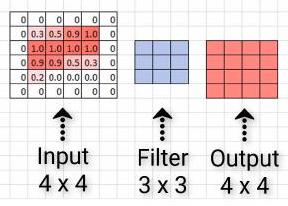
\includegraphics[max width=\textwidth]{2022_01_06_b5ce182ed1bd5f482e5bg-05}

\subsubsection{Convolution with stride (one channel)}
Definition 2. Convolution with stride 2 is defined as
$$
\left[K *_{2} g\right]_{i, j}=\sum_{p, q=-k}^{k} K_{p, q} g_{2 i+p-1,2 j+q-1}, \quad i=1:\left\lfloor\frac{m+1}{2}\right\rfloor, j=1:\left\lfloor\frac{n+1}{2}\right\rfloor
$$
We note that, in general, for any given integer $s \geq 1$, a convolution with stride $s$ for $g \in \mathbb{R}^{m \times n}$ can be defined as:
$$
\left[K *_{s} g\right]_{i, j}=\sum_{p, q=-k}^{k} K_{p, q} g_{s(i-11)+p+1, s(j-1)+q+1}, \quad i=1:\left\lfloor\frac{m+1}{s}\right\rfloor, j=1:\left\lfloor\frac{n+1}{s}\right\rfloor .
$$
Here $\left\lfloor\frac{m}{s}\right\rfloor$ denotes the biggest integer that less than $\frac{m}{s}$. The following is a diagram for stride 2 .

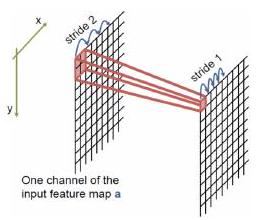
\includegraphics[max width=\textwidth]{2022_01_06_b5ce182ed1bd5f482e5bg-05(1)}

Lemma 1. The convolution with stride 2 can be written as:
$$
K *_{2} g=\mathcal{S}(K * g),
$$
where $\mathcal{S}$ is a stride operator defined by:
$$
\mathcal{S}: \mathbb{R}^{m \times n} \mapsto \mathbb{R}^{\frac{m+1}{2} \times \frac{n+1}{2}},
$$
with
$$
[\mathcal{S}(g)]_{i, j}=g_{2 i-1,2 j-1}, \quad i=1:\left\lfloor\frac{m+1}{2}\right\rfloor, j=1:\left\lfloor\frac{n+1}{2}\right\rfloor
$$
Example 1. The so-called average pooling with kernel size $3 \times 3$ and stride 2 means
$$
K *_{2},
$$
where
$$
K=\frac{1}{9}\left(\begin{array}{lll}
1 & 1 & 1 \\
1 & 1 & 1 \\
1 & 1 & 1
\end{array}\right)
$$

\subsubsection{Convolutional operations with multi-channel}
One important class of linear mapping is the so-called convolution:
$$
\theta: \mathbb{R}^{c \times m \times n} \mapsto \mathbb{R}^{h \times m \times n},
$$
where $m \times n$ is called the spatial dimension or resolution, $c$ and $h$ are corresponding to input and output channels. The operation is defined by
$$
[\theta(f)]_{s}=\sum_{t=1}^{c} K_{s, t} *[f]_{t}+b_{s} \mathbf{1} \in \mathbb{R}^{m \times n}, \quad s=1: h,
$$
where $1 \in \mathbb{R}^{m \times n}$ is a $m \times n$ matrix with all elements being 1 , and for $[f], \in \mathbb{R}^{m \times n}$ represent for the $t$-th channel
$$
\left[K_{s, t} *[f]_{t}\right]_{i, j}=\sum_{p, q=-k}^{k} K_{s, t ; p, q} f_{t ; i+p, j+q}, \quad i=1: m, j=1: n
$$
The coefficients kernel $K_{s, t}$ in (1.17) constitute a kernel matrix
$$
K_{s, t} \in \mathbb{R}^{(2 k+1) \times(2 k+1)}
$$
where $k$ is often taken as small integers.

Here a more compact notation for multi-channel convolution can be written as
$$
\theta(f)=K * f+\mathbf{b}
$$
where
$$
f=\left(\begin{array}{c}
{[f]_{1}} \\
{[f]_{2}} \\
\vdots \\
{[f]_{c}}
\end{array}\right), \quad K=\left(\begin{array}{cccc}
K_{1,1} & K_{1,2} & \cdots & K_{1, c} \\
K_{2,1} & K_{2,2} & \cdots & K_{2, c} \\
\vdots & \vdots & \ddots & \vdots \\
K_{h, 1} & K_{h, 2} & \cdots & K_{h, c}
\end{array}\right), \quad \mathbf{b}=\left(\begin{array}{c}
b_{1} \mathbf{1} \\
b_{2} \mathbf{1} \\
\vdots \\
b_{h} \mathbf{1}
\end{array}\right)=b \otimes 1
$$
Furthermore, we have the following natural extension of convolution with stride for multi-channel by
$$
[\theta(f)]_{s}=\sum_{t=1}^{c} K_{s, t} *_{2}[f]_{t}+b_{s} 1 \in \mathbb{R}^{\tilde{m} \times \tilde{n}}, \quad s=1: h,
$$
where
$$
\tilde{m}=\left\lfloor\frac{m+1}{2}\right\rfloor, \quad \tilde{n}=\left\lfloor\frac{n+1}{2}\right\rfloor
$$

\subsubsection{Pooling operation in CNNs}
Finally, we introduce another type of important operation in CNNs - pooling. The key purpose for pooling operator is to reduce the spatial resolution of images (features) in a typical CNN models. Basically, pooling is an operator
$$
T: \mathbb{R}^{c_{1} \times m_{1} \times n_{1}} \mapsto \mathbb{R}^{c_{2} \times m_{2} \times n_{2}} .
$$
where
$$
m_{2}=\left\lfloor\frac{m+1}{s}\right\rfloor, \quad n_{2}=\left\lfloor\frac{n+1}{s}\right\rfloor
$$
for any choice of $c_{2} \geq 1$. Here $s$ is also called the stride in pooling operations. There are generally two types of pooling

\section{Convolution with stride s as pooling}
In this case, it often happens that
$$
T=R *_{s}, \quad(s=2 \text { for the main case }) .
$$
Here $R$ can be learned or fixed such as average pooling as we discussed before.

\section{Nonlinear pooling}
The most commonly used nonlinear pooling is called max-pooling, a max pooling with kernel size $(2 k+1) \times(2 k+1)$ and stride $s$ is is defined as
$$
\left[R_{\max }(f)\right]_{t ; i, j}=\max \left\{f_{t ; s i+p-1, s j+q-1} \mid-k \leq p, q \leq k\right\}
$$
here $t$ means channel and $c_{2}=c_{1}$ in this case.

Here is an example for max-pooling with kernel size $2 \times 2$ and stride 2 .

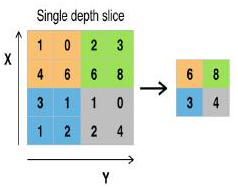
\includegraphics[max width=\textwidth]{2022_01_06_b5ce182ed1bd5f482e5bg-07}

\subsection{Examples of convolution filters and performance}
In this section, we will give a brief description how convolution operations are used for image processing. One useful description can be found in the following link:

\href{http://aishack.in/tutorials/image-convolution-examples/}{http://aishack.in/tutorials/image-convolution-examples/}

Convolutions is a technique for general signal processing. People studying electrical/electronics will tell you the near infinite sleepless nights these convolutions have given them. Entire books have been written on this topic. And the questions and theorems that need to be proved are [insurmountable]. But for computer vision, we'll just deal with some simple things.

A convolution lets you do many things, like calculate derivatives, detect edges, apply blurs, etc. A very wide variety of things. And all of this is done with a "convolution kernel"

\subsubsection{Calculation with convolutions}
The most direct way to compute a convolution would be to use multiple for loops. But that causes a lot of repeated calculations. And as the size of the image and kernel increases, the time to compute the convolution increases too (quite drastically).

Techniques haves been developed to calculate convolutions rapidly. One such technique is using the Discrete Fourier Transform. It converts the entire convolution operation into a simple multiplication. Fortunately, you don't need to know the math to do this in OpenCV. It automatically decides whether to do it in frequency domain (after the DFT) or not.

\subsubsection{Image convolution examples}
A convolution is very useful for signal processing in general. There is a lot of complex mathematical theory available for convolutions. For digital image processing, you don't have to understand all of that. You can use a simple matrix as an image convolution kernel and do some interesting things!

\subsubsection{Line detection by 1D Laplacian}
With image convolutions, you can easily detect lines. Here are four convolutions to detect horizontal, vertical and lines at 45 degrees:

Here's $0,90,45,135$ lines detection that I got on an image:
$$
\begin{array}{|c|c|c|}
\hline-1 & -1 & -1 \\
\hline 2 & 2 & 2 \\
\hline-1 & -1 & -1 \\
\hline
\end{array}
$$
$$
\begin{array}{|c|c|c|}
\hline-1 & 2 & -1 \\
\hline-1 & 2 & -1 \\
\hline-1 & 2 & -1 \\
\hline
\end{array}
$$
$$
\begin{array}{|c|c|c|}
\hline-1 & -1 & 2 \\
\hline-1 & 2 & -1 \\
\hline 2 & -1 & -1 \\
\hline
\end{array}
$$

\includegraphics[max width=\textwidth]{2022_01_06_b5ce182ed1bd5f482e5bg-09}

(a) image
$$
\left(\begin{array}{ccc}
-1 & -1 & -1 \\
2 & 2 & 2 \\
-1 & -1 & -1
\end{array}\right)
$$
(b) filter

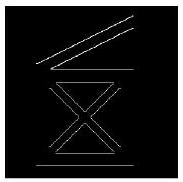
\includegraphics[max width=\textwidth]{2022_01_06_b5ce182ed1bd5f482e5bg-09(1)}

(c) result

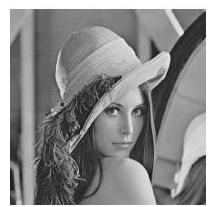
\includegraphics[max width=\textwidth]{2022_01_06_b5ce182ed1bd5f482e5bg-09(2)}

(d) image

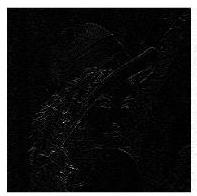
\includegraphics[max width=\textwidth]{2022_01_06_b5ce182ed1bd5f482e5bg-09(3)}

(e) result

Fig. 1.2. A horizontal line detection done with convolutions

In Lena, the black background is the original result, the white background is obtained by subtracting the original result from 255, the same below.


\includegraphics[max width=\textwidth]{2022_01_06_b5ce182ed1bd5f482e5bg-10}

(a) image

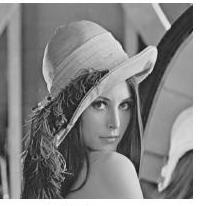
\includegraphics[max width=\textwidth]{2022_01_06_b5ce182ed1bd5f482e5bg-10(1)}

(d) image $\left(\begin{array}{lll}-1 & 2 & -1 \\ -1 & 2 & -1 \\ -1 & 2 & -1\end{array}\right)$

(b) filter

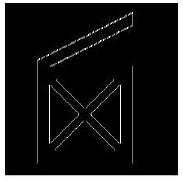
\includegraphics[max width=\textwidth]{2022_01_06_b5ce182ed1bd5f482e5bg-10(2)}

(c) result

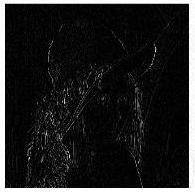
\includegraphics[max width=\textwidth]{2022_01_06_b5ce182ed1bd5f482e5bg-10(3)}

(e) result

Fig. 1.3. A vertical line detection done with convolutions


\includegraphics[max width=\textwidth]{2022_01_06_b5ce182ed1bd5f482e5bg-10(4)}

(a) image

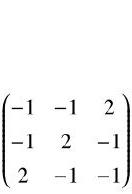
\includegraphics[max width=\textwidth]{2022_01_06_b5ce182ed1bd5f482e5bg-10(5)}

(b) filter (c) result

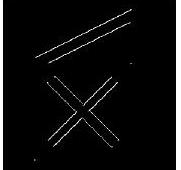
\includegraphics[max width=\textwidth]{2022_01_06_b5ce182ed1bd5f482e5bg-10(6)}

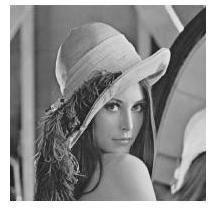
\includegraphics[max width=\textwidth]{2022_01_06_b5ce182ed1bd5f482e5bg-11}

(d) image

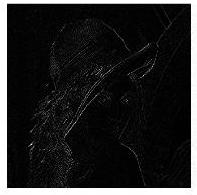
\includegraphics[max width=\textwidth]{2022_01_06_b5ce182ed1bd5f482e5bg-11(1)}

(e) result

Fig. 1.4. A 45 degress line detection done with convolutions


\includegraphics[max width=\textwidth]{2022_01_06_b5ce182ed1bd5f482e5bg-11(2)}

(a) image

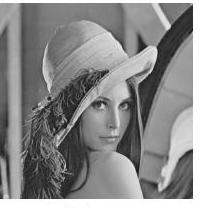
\includegraphics[max width=\textwidth]{2022_01_06_b5ce182ed1bd5f482e5bg-11(3)}

(d) image

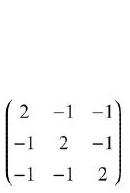
\includegraphics[max width=\textwidth]{2022_01_06_b5ce182ed1bd5f482e5bg-11(4)}

(b) filter

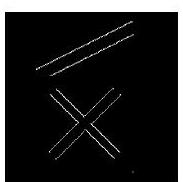
\includegraphics[max width=\textwidth]{2022_01_06_b5ce182ed1bd5f482e5bg-11(5)}

(c) result

Fig. 1.5. A 135 degress line detection done with convolutions

\subsubsection{Edge detection by 2D Laplacian operator}
The laplacian is the second derivative of the image. It is extremely sensitive to noise, so it isn't used as much as other operators. Unless, of course you have specific requirements.

\begin{tabular}{|c|c|c|}
\hline
0 & $-1$ & 0 \\
\hline
$-1$ & 4 & $-1$ \\
\hline
0 & $-1$ & 0 \\
\hline
\end{tabular}

\begin{tabular}{|c|c|c|}
\hline
$-1$ & $-1$ & $-1$ \\
\hline
$-1$ & 8 & $-1$ \\
\hline
$-1$ & $-1$ & $-1$ \\
\hline
\end{tabular}

The laplacian operator

(include diagonals)

Here's the result with the convolution kernel without diagonals:


\includegraphics[max width=\textwidth]{2022_01_06_b5ce182ed1bd5f482e5bg-12}

(a) image

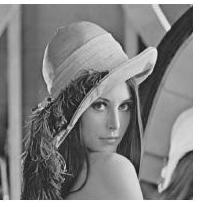
\includegraphics[max width=\textwidth]{2022_01_06_b5ce182ed1bd5f482e5bg-12(1)}

(d) image

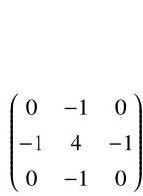
\includegraphics[max width=\textwidth]{2022_01_06_b5ce182ed1bd5f482e5bg-12(2)}

(b) filter

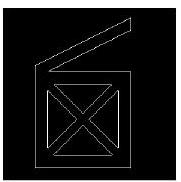
\includegraphics[max width=\textwidth]{2022_01_06_b5ce182ed1bd5f482e5bg-12(3)}

(c) result

Fig. 1.6. A laplace operator done with convolutions

The result with the convolution kernel with diagonals:


\includegraphics[max width=\textwidth]{2022_01_06_b5ce182ed1bd5f482e5bg-13}

(a) image

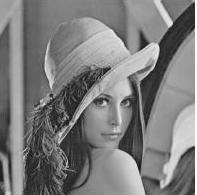
\includegraphics[max width=\textwidth]{2022_01_06_b5ce182ed1bd5f482e5bg-13(1)}

(d) image
$$
\left(\begin{array}{ccc}
-1 & -1 & -1 \\
-1 & 8 & -1 \\
-1 & -1 & -1
\end{array}\right)
$$
(b) filter

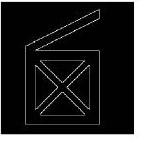
\includegraphics[max width=\textwidth]{2022_01_06_b5ce182ed1bd5f482e5bg-13(2)}

(c) result

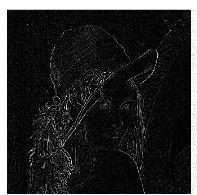
\includegraphics[max width=\textwidth]{2022_01_06_b5ce182ed1bd5f482e5bg-13(3)}

(e) result

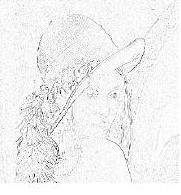
\includegraphics[max width=\textwidth]{2022_01_06_b5ce182ed1bd5f482e5bg-13(4)}

Fig. 1.7. A laplace operator include diagonals done with convolutions

\subsubsection{The Laplacian of Gaussian}
The laplacian alone has the disadvantage of being extremely sensitive to noise. So, smoothing the image before a laplacian improves the results we get. This is done with a $5 \times 5$ image convolution kernel.

\begin{tabular}{|c|c|c|c|c|}
\hline
0 & 0 & $-1$ & 0 & 0 \\
\hline
0 & $-1$ & $-2$ & $-1$ & 0 \\
\hline
$-1$ & $-2$ & 16 & $-2$ & $-1$ \\
\hline
0 & $-1$ & $-2$ & $-1$ & 0 \\
\hline
0 & 0 & $-1$ & 0 & 0 \\
\hline
\end{tabular}

The result on applying this image convolution was:


\includegraphics[max width=\textwidth]{2022_01_06_b5ce182ed1bd5f482e5bg-14}

(a) image

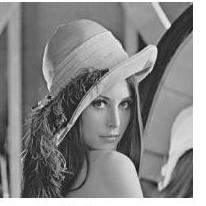
\includegraphics[max width=\textwidth]{2022_01_06_b5ce182ed1bd5f482e5bg-14(1)}

(d) image\\

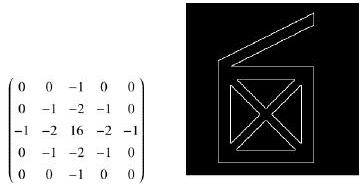
\includegraphics[max width=\textwidth]{2022_01_06_b5ce182ed1bd5f482e5bg-14(2)}

(b) filter

(c) result

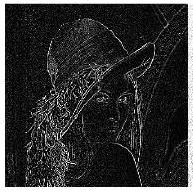
\includegraphics[max width=\textwidth]{2022_01_06_b5ce182ed1bd5f482e5bg-14(3)}\\

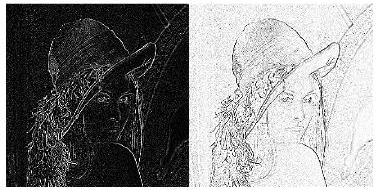
\includegraphics[max width=\textwidth]{2022_01_06_b5ce182ed1bd5f482e5bg-14(4)}

Fig. 1.8. A Laplacian of Gaussian operator done with convolutions

\subsubsection{Other examples with ReLU activation}
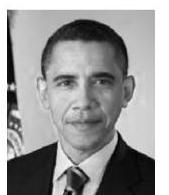
\includegraphics[max width=\textwidth]{2022_01_06_b5ce182ed1bd5f482e5bg-15}
$$
\left(\begin{array}{ccccc}
0 & 0 & -1 & 0 & 0 \\
0 & -1 & -2 & -1 & 0 \\
-1 & -2 & 16 & -2 & -1 \\
0 & -1 & -2 & -1 & 0 \\
0 & 0 & -1 & 0 & 0
\end{array}\right)
$$
(b) filter

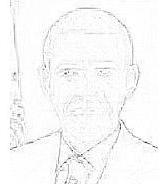
\includegraphics[max width=\textwidth]{2022_01_06_b5ce182ed1bd5f482e5bg-15(1)}

(c) convolution result

(a) input image

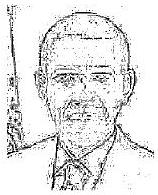
\includegraphics[max width=\textwidth]{2022_01_06_b5ce182ed1bd5f482e5bg-15(2)}

(d) result after ReLU $\left(\begin{array}{lll}\frac{1}{9} & \frac{1}{9} & \frac{1}{9} \\ \frac{1}{9} & \frac{1}{9} & \frac{1}{9} \\ \frac{1}{9} & \frac{1}{9} & \frac{1}{9}\end{array}\right)$

(e) filter

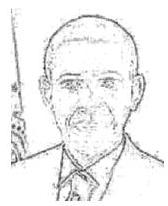
\includegraphics[max width=\textwidth]{2022_01_06_b5ce182ed1bd5f482e5bg-15(3)}

(f) result after average

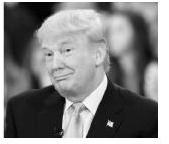
\includegraphics[max width=\textwidth]{2022_01_06_b5ce182ed1bd5f482e5bg-15(4)}

(g) image

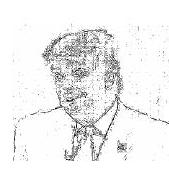
\includegraphics[max width=\textwidth]{2022_01_06_b5ce182ed1bd5f482e5bg-15(5)}

(j) ReLU
$$
\left(\begin{array}{ccccc}
0 & 0 & -1 & 0 & 0 \\
0 & -1 & -2 & -1 & 0 \\
-1 & -2 & 16 & -2 & -1 \\
0 & -1 & -2 & -1 & 0 \\
0 & 0 & -1 & 0 & 0
\end{array}\right)
$$
(h) filter

$\left(\begin{array}{lll}\frac{1}{9} & \frac{1}{9} & \frac{1}{9} \\ \frac{1}{9} & \frac{1}{9} & \frac{1}{9} \\ \frac{1}{9} & \frac{1}{9} & \frac{1}{9}\end{array}\right)$

(k) filter

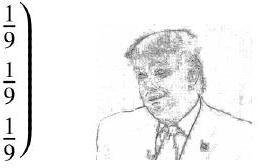
\includegraphics[max width=\textwidth]{2022_01_06_b5ce182ed1bd5f482e5bg-15(6)}

(1) average

\subsubsection{Some other examples}
\section{Edge detection}
The above kernels are in a way edge detectors. Only thing is that they have separate components for horizontal and vertical lines. A way to "combine" the results is to merge the convolution kernels. The new image convolution kernel looks like this:

\begin{tabular}{|r|l|l|}
\hline
$-1$ & $-1$ & $-1$ \\
\hline
$-1$ & 8 & $-1$ \\
\hline
$-1$ & $-1$ & $-1$ \\
\hline
\end{tabular}

Below result I got with edge detection:


\includegraphics[max width=\textwidth]{2022_01_06_b5ce182ed1bd5f482e5bg-16}

(m) image

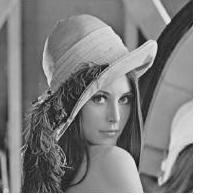
\includegraphics[max width=\textwidth]{2022_01_06_b5ce182ed1bd5f482e5bg-16(1)}

(p) image

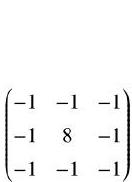
\includegraphics[max width=\textwidth]{2022_01_06_b5ce182ed1bd5f482e5bg-16(2)}

(n) filter

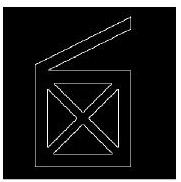
\includegraphics[max width=\textwidth]{2022_01_06_b5ce182ed1bd5f482e5bg-16(3)}

(o) result

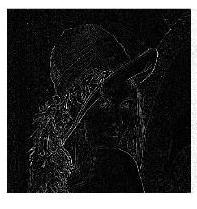
\includegraphics[max width=\textwidth]{2022_01_06_b5ce182ed1bd5f482e5bg-16(4)}

(q) result

Fig. 1.9. A edge detection done with convolutions

\section{The Sobel Edge Operator}
The above operators are very prone to noise. The Sobel edge operators have a smoothing effect, so they're less affected to noise. Again, there's a horizontal component and a vertical component.

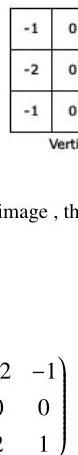
\includegraphics[max width=\textwidth]{2022_01_06_b5ce182ed1bd5f482e5bg-17}

\begin{tabular}{|c|c|c|}
\hline
$-1$ & $-2$ & $-1$ &  &  \\
\hline
0 & 0 & 0 &  &  \\
\hline
1 & 2 & 1 &  &  \\
\hline
\multicolumn{2}{|c|}{Horizontal} & $-1$ & 0 & 1 \\
\hline
$-2$ & 0 & 2 &  &  \\
\hline
$-1$ & 0 & 1 &  &  \\
\hline
\end{tabular}

On applying horizontal component in image, the result was:

\includegraphics[max width=\textwidth]{2022_01_06_b5ce182ed1bd5f482e5bg-17(1)}

(a) image

\includegraphics[max width=\textwidth]{2022_01_06_b5ce182ed1bd5f482e5bg-17(2)}

(d) image

\includegraphics[max width=\textwidth]{2022_01_06_b5ce182ed1bd5f482e5bg-17(3)}

(b) filter

\includegraphics[max width=\textwidth]{2022_01_06_b5ce182ed1bd5f482e5bg-17(4)}

(c) result

\includegraphics[max width=\textwidth]{2022_01_06_b5ce182ed1bd5f482e5bg-17(5)}

(e) result

Fig. 1.10. A horizontal sobel edge operator done with convolutions

On applying vertical component in image, the result was:

\includegraphics[max width=\textwidth]{2022_01_06_b5ce182ed1bd5f482e5bg-18}

(a) image

\includegraphics[max width=\textwidth]{2022_01_06_b5ce182ed1bd5f482e5bg-18(1)}

(d) image

\includegraphics[max width=\textwidth]{2022_01_06_b5ce182ed1bd5f482e5bg-18(2)}
$$
\left(\begin{array}{lll}
-1 & 0 & 1 \\
-2 & 0 & 2 \\
-1 & 0 & 1
\end{array}\right)
$$
(b) filter

\includegraphics[max width=\textwidth]{2022_01_06_b5ce182ed1bd5f482e5bg-18(3)}

(c) result\\

\includegraphics[max width=\textwidth]{2022_01_06_b5ce182ed1bd5f482e5bg-18(4)}

(e) result

Fig. 1.11. A vertical sobel edge operator done with convolutions

Fig. 1.11. A vertical sobel edge operator done with convolutions

\section{Simple box blur}
${ }^{1}$ Here's a first and simplest. This convolution kernel has an averaging effect. So you end up with a slight blur. The image convolution kernel is:
$$
\begin{array}{|l|l|l|}
\hline 1 / 9 & 1 / 9 & 1 / 9 \\
\hline 1 / 9 & 1 / 9 & 1 / 9 \\
\hline 1 / 9 & 1 / 9 & 1 / 9 \\
\hline
\end{array}
$$
Note that the sum of all elements of this matrix is $1.0$. This is important. If the sum is not exactly one, the resultant image will be brighter or darker.

Here's a blur that I got on an image:

$\overline{{ }^{1} \text { The following examples are from the website, http://aishack.in/tutorials/image- }}$ convolution-examples/

\includegraphics[max width=\textwidth]{2022_01_06_b5ce182ed1bd5f482e5bg-19}

(a) image

\includegraphics[max width=\textwidth]{2022_01_06_b5ce182ed1bd5f482e5bg-19(1)}

(b) filter

\includegraphics[max width=\textwidth]{2022_01_06_b5ce182ed1bd5f482e5bg-19(2)}

(c) result

\includegraphics[max width=\textwidth]{2022_01_06_b5ce182ed1bd5f482e5bg-19(3)}

(d) image

\includegraphics[max width=\textwidth]{2022_01_06_b5ce182ed1bd5f482e5bg-19(4)}

(e) filter

\includegraphics[max width=\textwidth]{2022_01_06_b5ce182ed1bd5f482e5bg-19(5)}

(f) result

Fig. 1.12. A simple blur done with convolutions

\section{Gaussian blur}
Gaussian blur has certain mathematical properties that makes it important for computer vision. And you can approximate it with an image convolution. The image convolution kernel for a Gaussian blur is:

\begin{tabular}{|l|l|l|l|l|l|l|}
\hline
0 & 0 & 0 & 5 & 0 & 0 & 0 \\
\hline
0 & 5 & 18 & 32 & 18 & 5 & 0 \\
\hline
0 & 18 & 64 & 100 & 64 & 18 & 0 \\
\hline
5 & 32 & 100 & 100 & 100 & 32 & 5 \\
\hline
0 & 18 & 64 & 100 & 64 & 18 & 0 \\
\hline
0 & 5 & 18 & 32 & 18 & 5 & 0 \\
\hline
0 & 0 & 0 & 5 & 0 & 0 & 0 \\
\hline
\end{tabular}

Here's a result that I got:

\includegraphics[max width=\textwidth]{2022_01_06_b5ce182ed1bd5f482e5bg-20}

(a) image

\includegraphics[max width=\textwidth]{2022_01_06_b5ce182ed1bd5f482e5bg-20(1)}

(d) image

\includegraphics[max width=\textwidth]{2022_01_06_b5ce182ed1bd5f482e5bg-20(2)}

(b) filter

\includegraphics[max width=\textwidth]{2022_01_06_b5ce182ed1bd5f482e5bg-20(3)}

(e) filter

\includegraphics[max width=\textwidth]{2022_01_06_b5ce182ed1bd5f482e5bg-20(4)}

(c) result

\includegraphics[max width=\textwidth]{2022_01_06_b5ce182ed1bd5f482e5bg-20(5)}

(f) result

Fig. 1.13. A Gaussian blur done with convolutions

\subsubsection{Summary}
You got to know about some important operations that can be approximated using an image convolution. You learned the exact convolution kernels used and also saw an example of how each operator modifies an image. I hope this helped!

\section{References}
[1] J. Deng, W. Dong, R. Socher, L.-J. Li, K. Li, and L. Fei-Fei. Imagenet: A largescale hierarchical image database. In 2009 IEEE conference on computer vision and pattern recognition, pages 248-255. Ieee, 2009.

[2] J. He, Y. Chen, and J. Xu. Constrained linear data-feature mapping for image classification. arXiv preprint arXiv: $1911.10428,2019 .$

[3] $\mathrm{K}$. He, X. Zhang, S. Ren, and J. Sun. Deep residual learning for image recognition. In Proceedings of the IEEE Conference on Computer Vision and Pattern Recognition, pages 770-778, 2016 .

[4] K. He, X. Zhang, S. Ren, and J. Sun. Identity mappings in deep residual networks. In European Conference on Computer Vision, pages 630-645. Springer, $2016 .$

[5] A. Krizhevsky and G. Hinton. Learning multiple layers of features from tiny images. Technical report, Citeseer, $2009 .$

[6] A. Krizhevsky, I. Sutskever, and G. E. Hinton. Imagenet classification with deep convolutional neural networks. In Advances in neural information processing systems, pages $1097-1105,2012$.

[7] Y. LeCun, L. Bottou, Y. Bengio, and P. Haffner. Gradient-based learning applied to document recognition. Proceedings of the IEEE, $86(11): 2278-2324,1998 .$

[8] K. Simonyan and A. Zisserman. Very deep convolutional networks for largescale image recognition. arXiv preprint arXiv: $1409.1556,2014 .$

[9] J. Xu and L. Zikatanov. Algebraic multigrid methods. Acta Numerica, 26:591$721,2017 .$


\end{document}